% !TEX root = EUDAQUserManual.tex
\section{Integration with User Hardware}\label{sec:Integration}
EUDAQ itself is only a data taking framework. It means that the users with their dedicated hardware and readout software are required to write some code to bridge the hardware specific readout software to the EUDAQ framework. The minimum adaptation task is to write a Producer for each piece of hardware, a Data Collector to receive the data (a.k.a.\ Event) from the Producers. 

\subsection{Announcement of Derived Class}
The derived EUDAQ classes provided by the user will be compiled and packed to a dynamic shared library (EUDAQ Module Library). At compiling/linking time of EUDAQ core library, it does not know of the existence of any Module Library. When the EUDAQ core library is being loaded by any application, the core library will look for any library file with the name prefix libeudaq\_module\_ in the module folder. All pattern matched libraries will be loaded. It is the point at which each derived EUDAQ class announces itself to the EUDAQ runtime environment.

Technically, the announcement of a derived class is done by a call to the correlated static function provided by a generic C++ template (eudaq::Factory). \autoref{tab:derivable} is the list of derivable EUDAQ classes.

\begin{table}
\centering
\small
\begin{tabular}{ l | l }
  \textbf{Class} & \textbf{Description}\\
  \hline
  \texttt{eudaq::Producer} & Sec. \ref{sec:ProducerWriting}\\
  \texttt{eudaq::DataCollector} & Sec. \ref{sec:DataCollectorWriting}\\
  \texttt{eudaq::RunControl} & Sec. \ref{sec:RunControlWriting}\\
  \texttt{eudaq::Event} &  Sec. \ref{sec:Event} \\
  \texttt{eudaq::LogCollector} & Sec. \ref{sec:logcollector} \\
  \texttt{eudaq::Monitor} & Sec. \ref{sec:MonitorWriting}\\
  \texttt{eudaq::FileWriter} & Sec. \ref{sec:FileWriterWriting}\\
  \texttt{eudaq::FileReader} & Sec. \ref{sec:FileReaderWriting}\\
  \texttt{eudaq::StdEventConverter} & Sec. \ref{sec:DataConverter} \\
  \texttt{eudaq::LCEventConverter} & Sec. \ref{sec:DataConverter} \\
  \texttt{eudaq::TransportServer} & internal only \\
  \texttt{eudaq::TransportClient} & internal only \\
\end{tabular}
\caption{Derivable Classes.}
\label{tab:derivable}
\end{table}

\subsection{Serializable}
As a distributed DAQ framework, a runtime setup of the EUDAQ system include several applications. Data objects will go through the boundary of an application or a computer. Those data objects should have the capability to be serialized. When a data object is serialized, all the crucial data of this data object is fed to serialized memory which then can be sent by plain binary to another application and reconstructed as a copy of the original data object. \\

All the classes which hold serializable data are derived from a base serializable class (eudaq::Serializable). All serializable data class
should implement the function \texttt{Serialize} which serializes the inner data object and feeds an eudaq::Serializer, and a constructor function which takes the reference of eudaq::Deserializer as input parameter.\\

\autoref{tab:serializable} is the list of serializable EUDAQ classes.

\begin{table}
\centering
\small
\begin{tabular}{ l | l }
  \textbf{Class} & \textbf{Description}\\
  \hline
  \texttt{eudaq::Event} & Sec. \ref{sec:Event} \\
  \texttt{eudaq::Configuration} & Contains configuration information \\
  \texttt{eudaq::LogMessage} & Messages reported to the LogCollector \\
  \texttt{eudaq::Status} & States reported to the RunControl \\
\end{tabular}
\caption{Serializable Classes.}
\label{tab:serializable}
\end{table}

\subsubsection{Event}\label{sec:Event}
eudaq::Event is most important serializable class which holds physics data from the hardware. The Producer is the EUDAQ component which creates the object eudaq::Event and feeds it the physics data from measurements.  \autoref{tab:eventdata} lists the variables inside the eudaq::Event. \\

\begin{table}
\centering
\small
\begin{tabular}{ l | l | l }
  \textbf{variable} & \textbf{C++ type} & \textbf{Description}\\
  \hline
  \texttt{m\_type} & \texttt{uint32\_t} & event type\\
  \texttt{m\_version} & \texttt{uint32\_t} & version\\
  \texttt{m\_flags} & \texttt{uint32\_t} & flags\\
  \texttt{m\_stm\_n} & \texttt{uint32\_t} & device/stream number\\
  \texttt{m\_run\_n} & \texttt{uint32\_t} & run number\\
  \texttt{m\_ev\_n} & \texttt{uint32\_t} & event number\\
  \texttt{m\_tg\_n} & \texttt{uint32\_t} & trigger number\\
  \texttt{m\_extend} & \texttt{uint32\_t} & reserved word\\
  \texttt{m\_ts\_begin} & \texttt{uint64\_t} & timestamp at the begin of event\\
  \texttt{m\_ts\_end} & \texttt{uint64\_t} & timestamp at the end of event\\
  \texttt{m\_dspt} & \texttt{std::string} & description\\
  \texttt{m\_tags} & \texttt{std::map<std::string, std::string>} & tags\\
  \texttt{m\_blocks} & \texttt{std::map<uint32\_t, std::vector<uint8\_t>>} & blocks of raw data\\
  \texttt{m\_sub\_events} & \texttt{std::vector<EventSPC>} & pointers of sub events\\
\end{tabular}
\caption{Variables of eudaq::Event.}
\label{tab:eventdata}
\end{table}

The \texttt{m\_blocks} is physics data which can only be known by the user who owns the hardware. There is a pair of timestamps to define the time slice when the physics event occurs, and a trigger number to identify the trigger sequence. Timestamps and trigger number are optional to be set if you are going to use them to synchronize data from multiple stream/device. It is also possible to have sub events inside an eudaq::Event object. The sub eudaq::Event objects are held by std::shared\_ptr, see the next section.

\subsection{Ownership}
std::shared\_ptr and std::unique\_ptr are heavily used in EUDAQ to hold the object pointers of the serializable class and the derivable class.  They get rid of the unnecessary and ineffective memory copy and are exception safe for any memory leakage.

\subsection{Command/Status Handling}
\subsubsection{RunControl and CommandReceiver}\label{sec:runcontrolrc}
\paragraph{RunControl} eudaq::RunControl is the command sender which issues commands according to user actions from the GUI or CLI.
\paragraph{CommandReceiver} eudaq::Producer, eudaq::DataCollector, eudaq::LogCollector and eudaq::Monitor are command receivers (eudaq::CommandReceiver) which executes the correlated function according to the command. The command receiver will set up a status (eudaq::Status) and report the status to RunControl.

\subsubsection{State Model}\label{sec:fsm}
\begin{figure}
\begin{center}
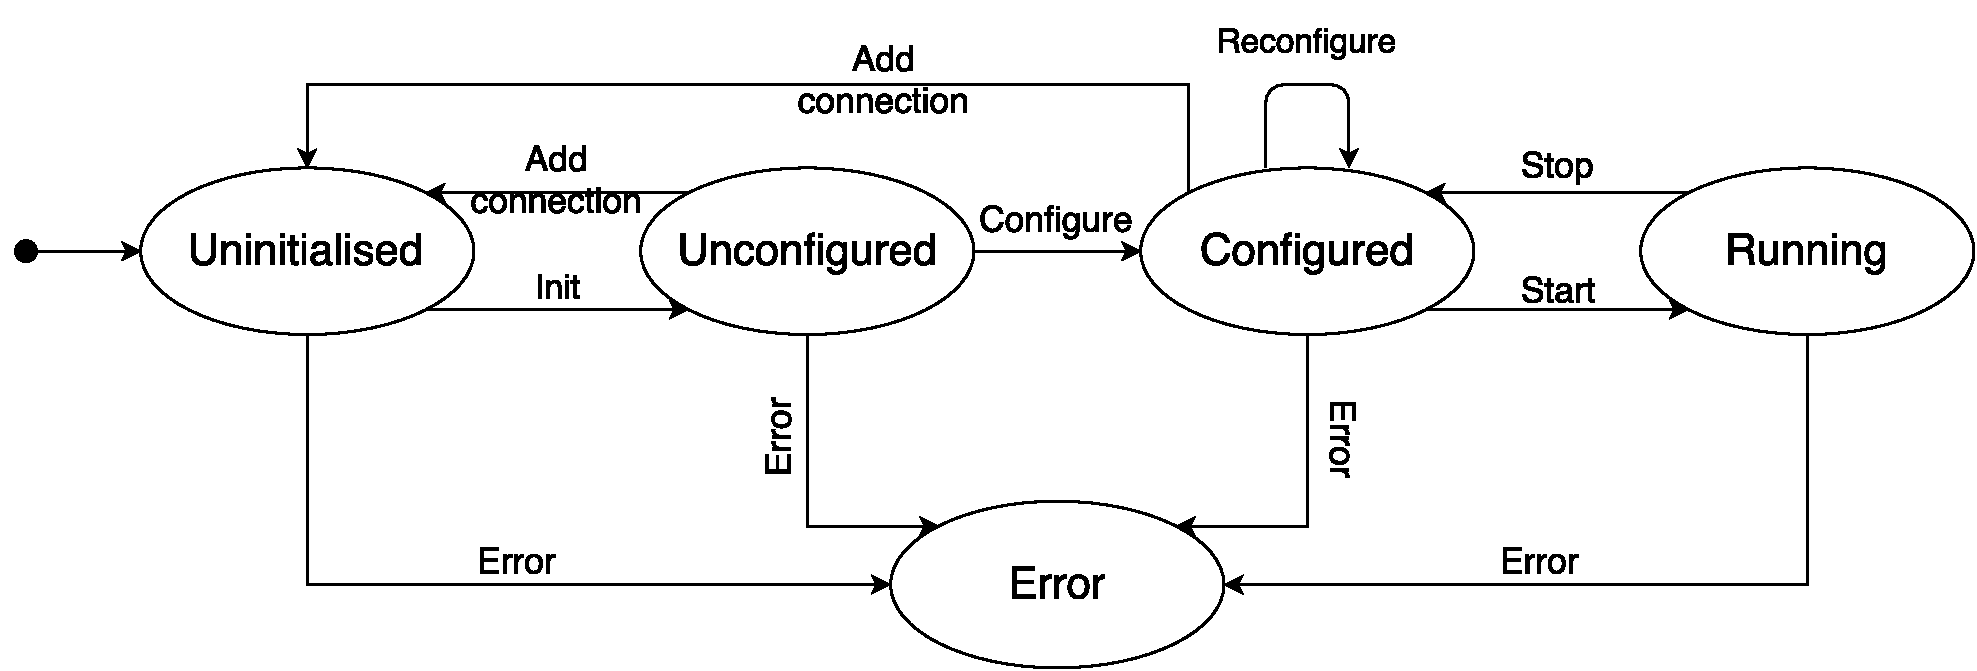
\includegraphics[width=0.9\textwidth]{src/images/fsmv2.pdf}
\end{center}
\caption{The FSM of EUDAQ.}
\label{fig:fsm}
\end{figure}

The \gls{FSM} is implemented in both the RunControl and the CommandReceiver (see \autoref{fig:fsm}) \cite{Shirokova:2016}. \\

Each CommandReceiver can always be characterized by the current state (\autoref{tab:statetab}).
\begin{table}
\centering
\small
\begin{tabular}{ l | l | l }
  \textbf{State} & \textbf{Enumerate Value} & \textbf{Acceptable Command} \\
  \hline
  \texttt{Error} & \texttt{eudaq::Status::STATE\_ERROR} & DoReset \\
  \texttt{Uninitialised} & \texttt{eudaq::Status::STATE\_UNINIT} & DoInitialise DoReset \\
  \texttt{Unconfigured} & \texttt{eudaq::Status::STATE\_UNCONF} & DoConfigure DoReset \\
  \texttt{Configured} & \texttt{eudaq::Status::STATE\_CONF} & DoConfigure DoStartRun DoReset \\
  \texttt{Running} & \texttt{eudaq::Status::STATE\_RUNNING} & DoStopRun \\
\end{tabular}
\caption{States of RunControl client.}
\label{tab:statetab}
\end{table}


The state of RunControl is determined by the lowest state of the connected client in the following priority: ERROR, UNINITIALISED, UNCONFIGURED, CONFIGURED, RUNNING. It means, for example, that even if only one connection is in the ERROR state, the whole machine will also be in that state. This prevents such mistakes as running the system before every component has finished the configuration.

\subsubsection{Command}\label{sec:command}

\begin{table}
\centering
\small
\begin{tabular}{ l | l | l | l |l }
  \textbf{Command} & \textbf{RunControl Side} & \textbf{Client Side} & \textbf{Pre State} & \textbf{State of Success}\\
  \hline
  \texttt{Initialise} & Initialise & DoInitialise & Uninitialised & Unconfigured\\
  \texttt{Configure} & Configure & DoConfigure & Unconfigured Configured & Configured\\
  \texttt{StartRun} & StartRun & DoStartRun & Configured & Running\\
  \texttt{StopRun} & StopRun & DoStopRun & Running & Configured\\
  \texttt{Reset} & Reset & DoReset & Error & Uninitialised\\
  \texttt{Terminate} & Terminate & DoTerminate & Any apart from Running & - \\
\end{tabular}
\caption{List of Commands.}
\label{tab:cmdtab}
\end{table}


\paragraph{Initialise}
When an EUDAQ process is in the state of Uninitialised, it accepts the Initialise command and executes the DoInitialise function provided by the user. When it is initialized, it does not accept further Uninitialised commands until it is reset to the Uninitialised state.

\paragraph{Configure}
When an EUDAQ process is in the state of Unconfigured or Configured, it accepts the Configure command and executes the DoConfigure function provided by the user. Please be aware that the second Configure command after a successful execution of the Configure command is allowed. It means the EUDAQ process is re-configurable but not re-initialisible.

\paragraph{StartRun}
When an EUDAQ process is in the state of Configured, it also accepts the StartRun command and executes the DoStartRun function provided by the user. In the case of the Producer, the Producer should talk to the hardware and produce and send Event data. In the case of the DataCollector, the DataCollector will get the Event stream from its connected Producer.

\paragraph{StopRun}
When an EUDAQ process is in the state of Running, it only accepts the StopRun command and executes the DoStopRun function provided by the user. RunControl will not send the StopRun command to the DataCollector until all Producers have returned from the DoStopRun function and feedback their status.

\paragraph{Reset}
In any case when an EUDAQ process goes to the state of Error, only the Reset command is allowed.

\paragraph{Terminate}
Except for the state of Running, the terminate command is allowed on all other states. When the Terminate command is called, the EUDAQ processes will be closed. If the user has to do something before exiting the EUDAQ process, this should be entered into the DoTerminate function which will then carry out the process before exiting.

